\begin{minipage}{.5\textwidth}
    \centering
    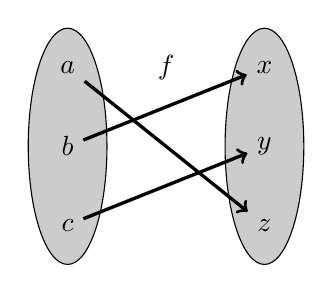
\begin{tikzpicture}[scale=0.5]
        \filldraw (1,3)[fill=black!20!white] circle [x radius=1cm, y radius=3cm];
        \filldraw (6,3)[fill=black!20!white] circle [x radius=1cm, y radius=3cm];
    
        \draw (3.5,5) node {$f$};
    
        \draw (1,5) node(a) {$a$};
        \draw (1,3) node(b) {$b$};
        \draw (1,1) node(c) {$c$};
    
        \draw (6,5) node(x) {$x$};
        \draw (6,3) node(y) {$y$};
        \draw (6,1) node(z) {$z$};
    
        \draw[->,very thick] (a) -- (z);
        \draw[->,very thick] (b) -- (x);
        \draw[->,very thick] (c) -- (y);
    \end{tikzpicture}
\end{minipage}%
\begin{minipage}{.5\textwidth}
    \centering
    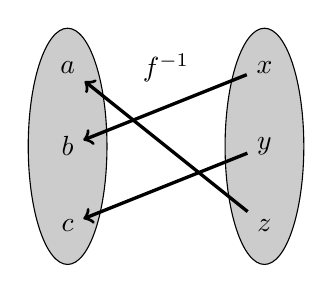
\begin{tikzpicture}[scale=0.5]
        \filldraw (1,3)[fill=black!20!white] circle [x radius=1cm, y radius=3cm];
        \filldraw (6,3)[fill=black!20!white] circle [x radius=1cm, y radius=3cm];
    
        \draw (3.5,5) node {$f^{-1}$};
    
        \draw (1,5) node(a) {$a$};
        \draw (1,3) node(b) {$b$};
        \draw (1,1) node(c) {$c$};
    
        \draw (6,5) node(x) {$x$};
        \draw (6,3) node(y) {$y$};
        \draw (6,1) node(z) {$z$};
    
        \draw[<-,very thick] (a) -- (z);
        \draw[<-,very thick] (b) -- (x);
        \draw[<-,very thick] (c) -- (y);
    \end{tikzpicture}
\end{minipage}
